\section{Results}
\label{sec:results}

The primary experiment is the Class~A search for a drifting, unresolved
spectral carrier: \NWinA{} fine-channel windows toward \NSysClassA{}
systems. The Class~B search for an unresolved spectral excess is secondary
and carries no drift discrimination: \NWinB{} coarse windows. Together they
are the \NWindows{} windows of the released catalogue. \textbf{No carrier
was found toward any of the \NSystems{} systems searched.} What follows is
first how deep the search reaches, and then what it found and how each
finding was disposed of.

\subsection{Sensitivity: the power at which a carrier would have been
found} \label{sec:pninetysel}

\emph{The sensitivity of this survey is a measured completeness and not a
threshold.} Artificial carriers were added to the real calibrated
visibilities, each at a random sub-channel phase and with a random drift rate
from its window's own grid, and recovered through the unchanged pipeline:
extraction, baseline removal, de-drifted stack, trigger and the
\NCtrl-position spatial screen. The power at which nine carriers in ten come
back is $\mathrm{EIRP}_{90}$, the only sensitivity quoted here. It charges
for the whole chain, because a carrier counts as recovered only when it
reaches the trigger \emph{and} outranks every control.

\emph{Measured that way the completeness is not one number, and what it
depends on is the control ring.} In the \StrNNoiseWin{} of \NWinA{} Class~A
windows whose ring is noise, nine carriers in ten are recovered at
$\StrMultNoise\,P_{\rm trig}$, where $P_{\rm trig}$ is that window's own
trigger power. In the other \StrNDiscWin, toward \StrDiscStars,
the ring carries resolved disc emission; a carrier there has to outshine the
star's own surroundings rather than the noise, and the injected ladder never
reaches ninety per cent below $\StrTopRung\,P_{\rm trig}$, although every
carrier is recovered by $\StrPosCtrl\,P_{\rm trig}$. The second figure is
therefore a bound and not a value, and each window is quoted on the stratum
it belongs to. A single factor fitted to both strata together would be
$\EirpNinetyMultA$, and that is the completeness of no window in the survey:
it sits above the first stratum's own spread and far below the second's
bound. Class~B keeps one factor, $\EirpNinetyMultB\,P_{\rm trig}$: no
injected coarse window has a bright ring, so the distinction cannot be
measured there and the \StrNBrightB{} coarse windows that do are flagged in
the catalogue instead.

\emph{Separating the two strata moves power between windows; it does not
make the survey better.} The median Class~A window reaches
$\EirpNinetyWinMedA$\,W of equivalent isotropic radiated power and the median
system, on its best window, $\EirpNinetySysMedA$\,W, with a spread across
systems of $\EirpNinetySysLoA$--$\EirpNinetySysHiA$\,W
(Fig.~\ref{fig:classasens}a). The round $10^{15}$\,W level is reached for
\NSysEfifteen{} of them. Against a single blanket factor those limits are about a fifth
deeper for \StrNNoiseWin{} windows and several times shallower for
\StrNDiscWin, and the worst-placed system in the survey moves the wrong way
because its best window is one of them. A second term runs against us
throughout: the assumed phase centre omits the annual parallax, so a nearby
star observed in a long-baseline configuration loses amplitude. The loss is
\PxaLossMedPct{} per cent in the median window and \PxaLossMaxPct{} per cent
at worst, passing a tenth in \PxaNGtTen{} of the \PxaNWin{} windows that
carry the astrometric keys, and dividing each window by the fraction it
retains makes every limit shallower --- the median Class~A limit by
\PxaShiftWinPct{} per cent. One window, \PxaMissingStar{} in \PxaMissingEb,
has no such keys and is left uncorrected.
Table~\ref{tab:p90budget} collects these signed terms and the two-sided ones,
which combine to $\times\EirpNinetyFacLo$--$\times\EirpNinetyFacHi$ on every
limit.

\emph{Carriers were injected directly into \BudTransN{} Class~A windows and
the result transferred to the remaining \BudTransNTransferred, which is the
dominant caveat on all of the above.} Figure~\ref{fig:strata}(a) shows the
individual measurements rather than their summary: \StrNIndiv{} of the
\StrNInjWin{} resolve a ninety per cent point, between $\StrIndivLo$ and
$\StrIndivHi\,P_{\rm trig}$, and the three that do not are the
brightest-ring windows of all. There is no dependence on observing band or
on channel width, the median values differing by \StrBandSpread{} and
\StrChanSpread. There is an apparent difference between the two arrays,
$\StrArrTwelve$ against $\StrArrAca$, and it is not the array: it is carried
by \StrNArrDriver{} windows whose target has bright emission near the ring,
and it falls to $\StrArrTwelveSub$ against $\StrArrAcaSub$ once the star's
own leak into the control positions is removed. That is why the strata are
cut on the ring. Removing the leak is a diagnostic and not the screen we
apply, since it would make the test for a source depend on a model of that
source; and it buys little, moving the noise-dominated figure to
$\StrMultNoiseSub$ and the disc-affected windows not at all, because there
the ring is set by the disc. Only the distance is worse for a single star than for
the sample: of the \BudPlxNStar{} Gaia parallaxes the worst fractional error
is \SfPlxWorstPct{} per cent, toward \SfPlxWorstStar.

\begin{table}
\centering
\scriptsize
\caption{What sets $\mathrm{EIRP}_{90}$, and in which direction. The
two-sided terms combine in quadrature to one interval applying to every
limit; the signed terms are biases, stated with their direction rather than
folded into an error bar. The channel response is carried by the injections
rather than applied afterwards: at the ninety per cent point the recovered
peak channel holds $\InjPeakAtNinety\times$ the nominal trigger, so the
response is already inside the measured completeness and applying it again
would count it twice.}
\label{tab:p90budget}
\tiny
\setlength{\tabcolsep}{2pt}
%% GENERATED by numbers_v410.py -- do not hand-edit.
\begin{tabular}{@{}l@{~~}r@{~~}>{\raggedright\arraybackslash}p{0.38\columnwidth}@{}}
\hline
 & value & what it does to the limit \\
\hline
\multicolumn{3}{@{}l}{\emph{Measured completeness}, as a multiple of a window's own trigger power} \\
Ring is noise (390 windows) & $\times3.45$ & measured; $\times3.37$--$\times4.20$ across resamples \\
Ring carries emission (12) & $>\times8$ & a bound: everything is recovered by $\times20$, nothing at the trigger \\
One factor for both & $\times4.42$ & the completeness of no window; not used \\
\hline
\multicolumn{3}{@{}l}{\emph{Two-sided uncertainties} (per cent), combined in quadrature} \\
Window-to-window transfer & $-22/+8$ & the spread across the 21 injected windows \\
Flux, distance and visibility scale & $\pm9$ & calibration \\
\emph{Combined} & $-23/+12$ & $\times0.77$--$\times1.12$ on every limit \\
\hline
\multicolumn{3}{@{}l}{\emph{Signed terms}. A bias is not an error bar and is not added to one.} \\
Channel response & $\times2.3$ & carried by the injections, so already inside the completeness above \\
\quad its residual & $+8$ & the injected profile falls short of the exact response: \emph{conservative} \\
Phase centre, annual parallax & $+1.5$ & applied window by window; every limit \emph{shallower} \\
Decorrelation & $-12/+17$ & declared from the literature, not measured here \\
\hline
\end{tabular}

\end{table}

\begin{figure*}
\centering
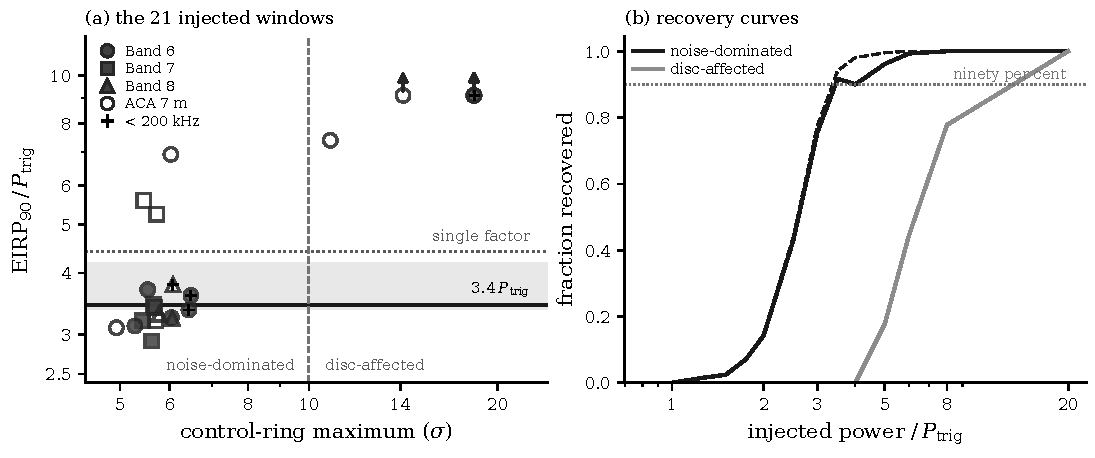
\includegraphics[width=0.94\textwidth]{figures/sens_strata.pdf}
\caption{Why the completeness is quoted in two strata. \emph{(a)}~The
\StrNInjWin{} directly injected Class~A windows, each at the power that
recovers nine carriers in ten, against the maximum of its own control ring.
Marker shape is the band, open symbols the compact array, a cross a channel
narrower than 200\,kHz, and arrows the three windows that never reach ninety
per cent. The line and band are the noise-dominated value and its spread,
the dotted line the single factor fitted to all of them. \emph{(b)}~The two
strata's recovery curves: solid as the screen is applied, dashed with the
star's own leak into the ring removed, which is a diagnostic and not the test
used here. The disc-affected pair lie on top of one another.}
\label{fig:strata}
\end{figure*}

\begin{figure*}
\centering
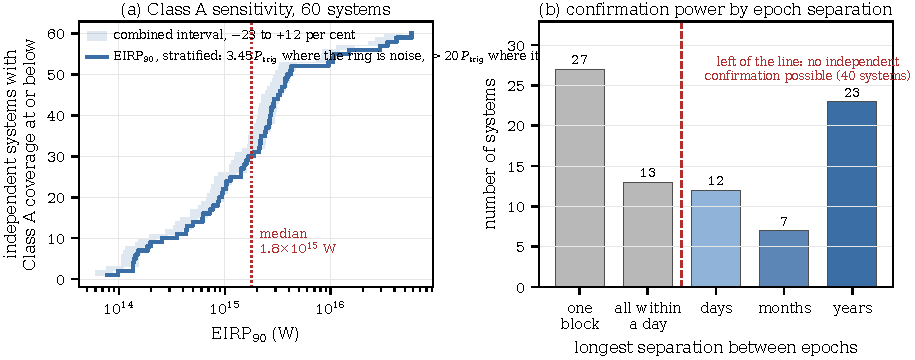
\includegraphics[width=0.92\textwidth]{figures/classa_sensitivity.pdf}
\caption{\emph{(a)}~Class~A sensitivity: the cumulative number of systems
whose best window reaches a given $\mathrm{EIRP}_{90}$, the power at which
nine carriers in ten are recovered through the trigger and the spatial
screen together. The shaded band is the combined interval of
Table~\ref{tab:p90budget}. \emph{(b)}~The temporal selection function:
systems grouped by the longest separation between their searched epochs, an
independent epoch being a separation of more than \EpSep{} day.
\textbf{For the \EpOne{} systems observed in a single block, and the
\EpSameDay{} whose blocks all fall within one day --- left of the dashed
line --- independent confirmation was not possible at all}, whatever the
sensitivity in panel~(a). Recurrence over years can be tested for
\EpYears{} systems of \EpTot.}
\label{fig:classasens}
\end{figure*}

\subsection{The nearest stars: Barnard's Star and Wolf~359}
\label{sec:barnardswolf}

Barnard's Star is the second-nearest stellar system, and Wolf~359 the third
if brown dwarfs are excluded. To our knowledge these are the first
millimetre or submillimetre technosignature limits for either; the searches
checked are \citet{Enriquez2017}, \citet{Price2020} and
\citet{Margot2023}. Both are non-detections. \emph{Both limits come from the
secondary Class~B experiment and not from the carrier search}: the archive
holds only coarse Band~6 windows toward these two stars, so neither is
searched for a drifting carrier and neither constrains one. What is
constrained is an unresolved spectral excess. Quoted on the
$\mathrm{EIRP}_{90}$ convention of \S\ref{sec:pninetysel}, Barnard's Star
reaches $\EirpNinetyBarnLo$--$\EirpNinetyBarnHi$\,W over \NWinBarn{}
windows. Wolf~359 reaches
$\EirpNinetyWolfLo$--$\EirpNinetyWolfHi$\,W over \NWinWolf.

\subsection{Threshold crossings and how each was disposed of}
\label{sec:technosearch}

\emph{The result is a chain of four tests, and it is read in one direction.}
Of the \NWindows{} windows, \NCross{} contain a channel\,$\times$\,drift
cell at the stellar position reaching $T\geq5$. Such a cell is a
\emph{threshold crossing}. The molecular-line mask,
$\pm\MaskHalfKms$\,km\,s$^{-1}$ wide, evaluated in each star's own rest
frame and fixed before any crossing was classified, identifies
\NAttributed{} of them with a catalogued transition.
\NUnattributed{} are unattributed by that test, and every crossing is in one
column or the other. Of the unattributed, \NUnattrRankFlagged{} outranks
all \NCtrl{} control positions in its own window, and it does not recur in
any later epoch covering its frequency. \textbf{No crossing survives the
chain, and this survey reports no detection.}
Figure~\ref{fig:chain} carries the chain with the number surviving each
step and Table~\ref{tab:ledger} the crossing-by-crossing ledger behind it.
%% v4.11 LENGTH (Ruling 4): tab:ledgersum is DELETED.  The sentence above
%% used to introduce it as "the same five counts" as the figure beside it and
%% the ledger below it -- three presentations of one result, which is the one
%% thing Ruling 4 forbids.  The five counts are macros and are stated in the
%% prose above; the fragment is still generated for the deposit.

\emph{The mask is informative rather than permissive, and its half-width is
not a tuned parameter.} The width follows from the Keplerian velocity bound
on circumstellar gas in these systems, and Table~\ref{tab:maskrobust}
carries every count in the chain above at half-widths from
$\pm\FrLadderLo$ to $\pm\FrLadderHi$\,km\,s$^{-1}$: the number outranking
every control is the same at all of them, and it is the same crossing. The
mask attributes \NAttributed{} crossings where its occupancy of the searched
band would give \LgExpAttr{} by chance alone, so the attributions are a
kinematic result and not an accident of bandwidth.

\subsubsection{Most of the crossings are expected by chance}
\label{sec:trigunif}

The trigger is a threshold on a statistic and not a false-alarm
rate: the number of searched channel\,$\times$\,drift cells per window spans
several decades, so a common threshold buys very unequal protection.
Summing each window's own measured false-alarm probability over the covered
Class~A windows gives \RsevChanceExp{} expected unattributed Class~A
crossings, against \RsevChanceObsAUnattr{} observed. \emph{About two thirds
of the crossings this survey reports are expected by chance}, which is why
the chain never treats a crossing as a detection and why no artefact
hypothesis is needed to account for their number.

\subsubsection{One execution block accounts for four of the crossings}
\label{sec:bdblock}

\BdNCross{} crossings belong to \BdStar{} (\BdAlias), with the highest
statistics in the survey outside $\beta$~Pictoris and HD~48370. All
\BdNCrossBlock{} lie in one ACA execution block, \texttt{\BdBlock}, in which
the whole field is above threshold: \BdNCtrlAbove{} of \BdNCtrl{} control
positions exceed $T=5$, against a survey median control maximum of
\BdSurvCtrlMed. The single-integration noise is as predicted
(\BdRmsMeas\,Jy against \BdRmsPred\,Jy), but the residual does not integrate
down; a jackknife on the channel mean gives \BdJack\,Jy against
\BdThermal\,Jy thermal. A slow drift common to every channel and every
position therefore inflates the statistic across the field. The
\BdNSibling{} sibling executions of the same field, with the same array and
the same spectral setup, reach a maximum of $T_\star=\BdSibTMax{}$ and
produce no crossing. \emph{The median of the control ensemble, not its
maximum, is the quality criterion this kind of search needs.} We report it
as a diagnostic and do not adopt it as a cut, because a cut strict enough to
remove this block would also remove the HD~48370 carbon-monoxide control.

\subsubsection{Stellar flares are excluded by a broadband prediction}

The hosts are not a quiet sample: \HostActiveClause, and magnetically
active stars do produce coherent
bursts at centimetre wavelengths. A millimetre flare, however, raises every
channel of a window by the same flux density. A flare able to produce a
single-channel crossing at the trigger must therefore produce a
$5\sqrt{N}\sigma$
continuum event in the same integrations. Over the \FlNCont{} crossings with
a recoverable continuum measurement that prediction runs
\FlPredLo--\FlPredHi$\sigma$, while the observed continuum statistic has
median \FlObsMed{} and $|Z|<3$ in \FlNQuiet{} of \FlNCont. One block settles
it directly. \FlEgStar{} \texttt{\FlEgEb} contains both a crossing
($T_\star=\FlEgT$) and the published millimetre flare of
\citet{MacGregor2020}. In the crossing's own time window the continuum is
raised at $Z=\FlEgContZ$, while the crossing's de-drifted track reaches only
$Z_{\max}=\FlEgTrackZ$. \emph{A real, bright, independently published
millimetre flare in the same data contributes \FlEgContrib$\sigma$ to the
single-channel statistic.}

\subsection{$\beta$~Pictoris: an astrophysical positive control, and the
obstacle it identifies} \label{sec:bpicval}

\emph{A search that finds nothing must show that it could have found
something, and the survey's strongest features show exactly that.} The
frozen pipeline recovers the $\beta$~Pictoris circumstellar carbon monoxide
blind, without being told the disc is there. It recovers it in two
rotational transitions and in \NStageOneBpicEb{} independent execution
blocks spanning \BpBaselineYr\,yr: \BpicNFlagThree{} Band~3 windows at
$T_\star$ up to \BpicBThreeTsym, and \BpicNFlagSix{} Band~6 windows at
\BpicBSixTsym. The identification is kinematic and does not rest on those
statistics. Carried through the frame chain --- to the barycentre at each
block's own epoch, then to the star's rest frame --- all \BpicPanelNCo{}
crossings lie within \BpicDvCoHi\,km\,s$^{-1}$ of the stellar systemic
velocity, in the two lowest CO transitions of a star with mapped
circumstellar CO \citep{Dent2014,Matra2017}. The Band~3 peaks agree across blocks to
\BpRecThreeTuneChanMax{} channel once each block's own tuning is removed, so
any apparent drift is far below the grid searched. The alternative reading
requires a transmitter placed by coincidence at matched offsets from two CO
transitions of one star.

$\beta$~Pictoris is also the control that shows the recurrence test of
\S\ref{sec:etacrv} working in the positive direction. Every
$\beta$~Pictoris carbon-monoxide feature the search flagged is recovered in
an independent execution block, and the screened Band~6 window returns
$T_\star=\BpRecTTwo{}$ in the second block of its own recurrence set. A
non-recurrence elsewhere means nothing unless the same machinery recovers a
repeat where one exists.

\emph{One of those blocks is a counterexample, and it is the more useful
half of the control.} In it the control ring is brighter than the star, and
several of the \NCtrl{} control positions exceed the stellar statistic, so
the spatial screen rejects a window containing carbon monoxide that is known
to be real and known to be centred on the star. The disc is resolved on the
scale of the primary beam in that configuration, which is exactly the
geometry the screen is built to reject. \textbf{The screen is therefore not
a test of authenticity but a test of compactness}, and on a real,
spatially extended source it fails in the conservative direction. That is a
stronger statement than a clean positive control would be, because it bounds
the screen's reach as well as demonstrating it (Fig.~\ref{fig:bpiccontrol}).

\begin{figure}
\centering
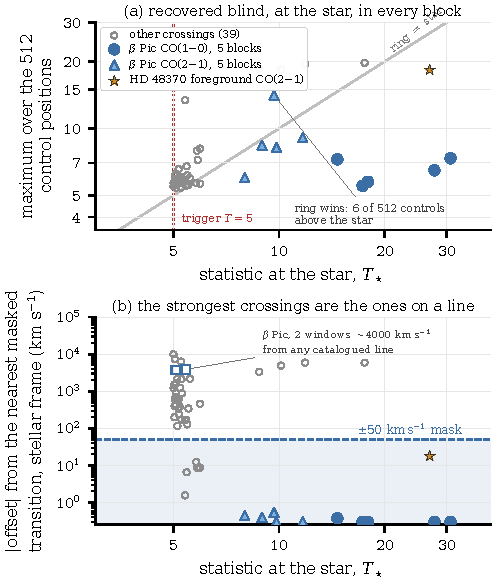
\includegraphics[width=0.88\columnwidth]{figures/bpic_control.pdf}
\caption{The $\beta$~Pictoris positive control, in both directions.
\emph{(a)}~The spatial screen. One point per execution block in which the
blind search recovers circumstellar carbon monoxide, plotted as the stellar
statistic against the maximum over that window's \NCtrl{} control positions:
the \NStageOneBpicEb{} blocks in which the star outranks every control, and
one further block in which the ring wins. \emph{The control is that the
search recovers a real narrow line at a stellar position, in two transitions
and in every one of these blocks.} It is not that the star outranks the ring
everywhere. In block \texttt{\BpCtrlBlock}, Band~\BpCtrlBand, the control
ring reaches \BpCtrlRingMax{} against \BpCtrlStar{} at the star, with
\BpCtrlNAbove{} of the \BpCtrlNCtrl{} control positions above it, so the
screen rejects a window holding carbon monoxide that is real, centred on the
star and independently mapped. The disc is resolved on the scale of the
primary beam in that configuration, which is the geometry the screen is
built to reject, so \textbf{the screen measures compactness and not
authenticity} (\S\ref{sec:bpicval}). \emph{(b)}~Line confusion, which is
what makes the screen's job hard. Each crossing is plotted by its velocity
offset from the nearest masked transition \emph{in its own star's rest
frame}, with the adopted $\pm\MaskHalfKms$\,km\,s$^{-1}$ half-width
marked. The \BpicPanelNCo{} $\beta$~Pictoris carbon-monoxide crossings land
\BpicDvCoLo--\BpicDvCoHi\,km\,s$^{-1}$ from CO, at the resolution of the
systemic velocity itself, while the two CS($5{\to}4$) crossings of the same
star sit \BpicDvCsLo--\BpicDvCsHi\,km\,s$^{-1}$ from anything catalogued
and are not attributed at any width. \BpicPanelNOther{} further crossings
are drawn in grey, with HD~48370 marked; \BpicPanelNDrawn{} of the
\NCross{} are plotted, the remainder being crossings for which the release
stores no control ring. \emph{A crossing is identified by where it falls in
this plane and not by how strong it is}, which is why the line mask and not
the trigger is the productive test.}
\label{fig:bpiccontrol}
\end{figure}

HD~48370 is the complementary case and is equally instructive. Its crossing
reaches $T_\star=\HdTsym$, but the control ring rises with the star, to
\HdRingMax, as emission filling the primary beam does. The velocity matches
the prominent CO($2{\to}1$) that \citet{Cataldi2023} report toward the
source and flag as possible foreground cloud emission. The block's
$^{13}$CO($2{\to}1$) window is bright at the ring and faint at the star.
Extended line emission is therefore rejected by the same spatial statistic
that promotes $\beta$~Pictoris.

\emph{Taken together, these two results identify the dominant obstacle for
millimetre technosignature searches, and it is not sensitivity.} The
strongest apparent signals in this survey are circumstellar and foreground
molecular emission, and \NAttributed{} of the \NCross{} crossings land on a
catalogued transition. The mask that removes them costs \FrMaskPct{} per
cent of the unique-frequency union over \FrNSpec{} species, and it is
nevertheless the single most productive test in the chain. The warning for
future work is about line lists rather than about depth, and
Appendix~\ref{app:linemask} puts a number on it.

\subsection{The crossings that survive the line mask}
\label{sec:chaingap}

\NUnattrRankFlagged{} of the \NCross{} crossings is both unattributed and
outranks every one of the \NCtrl{} control positions in its own window:
\RcSxStar{} at \RcSxFreq\,GHz, in Band~\RcSxBand. The event closest to it in
the ledger, \RcCpStar{} at \RcCpFreq\,GHz, lies \RcCpDv\,km\,s$^{-1}$ from
\RcCpLine{} in the star's own frame, and the mask therefore attributes it.
These are the two most interesting events in the experiment, and everything
measured about them is in Table~\ref{tab:cand} rather than scattered through
the text.

\emph{Both are absent when the same frequency is observed again.}
\RcCpStar{} is the cleaner case. The next observation of that frequency began
\RcCpNearH\,hours later and is deeper; a carrier persisting at the discovery
flux would have returned $T_\star=\RcCpTPers$ there, and the value measured at
the predicted cell is \RcCpTObs. That excludes a persistent source at
\RcCpExcl$\sigma$ --- from a repeat two hours later, with no appeal to a line
list, a rank or a model. \RcSxStar{} has \RcSxNRep{} covering repeat blocks of
the \RcSxNCat{} the catalogue records, the nearest \RcSxNearH\,hours away,
expected $T_\star=\RcSxTPers$ against \RcSxTObs{} measured: \RcSxExcl$\sigma$.
Neither is carried forward.

\subsubsection{The visibility fit, and why it is not the discriminant}
\label{sec:vistest}

\LgNFit{} of the \NCross{} crossings were re-measured in the visibility
domain, by phase rotating to the star and following the recovered drift
(Table~\ref{tab:visfit}). The result sits beside the chain rather than inside
it because a noise maximum \emph{at} the stellar position has flux at the
stellar position: at the trigger the fit returns a real part close to the
trigger itself and adds little to the trigger that selected it. Injected
sources in the bin the unattributed crossings occupy return
${\rm Re}/\sigma=\RsevReAtFiveMeanA\pm\RsevReAtFiveSdA$, and the two events
above are consistent with a real source and do not exclude one.
\textbf{The discriminating evidence is the line mask and recurrence.}

\subsection{Recurrence, applied to every unattributed crossing}
\label{sec:etacrv}

\emph{A persistent transmitter should be there the next time the same
frequency is observed.} That is the confirmation criterion, applied in the
star's own frame: the expected channel follows from the Earth's motion at the
repeat epoch and the star's systemic velocity, the discovery drift is
transported to it, and the survey's own statistic is read at that one cell.
Nothing is maximised, so what comes back is an amplitude with an uncertainty.

The test is run on \emph{every} unattributed crossing with any covering repeat
coverage, and not only on those that outrank their controls: the control rank
has no calibrated false-alarm probability, so it cannot be allowed to decide
which crossings are tested. \RcNTested{} of the \NUnattributed{} were tested,
over \RcNRepeatMeas{} covering repeat windows in \RcNRepeatBlock{} execution
blocks, \RcNRepeatFollow{} of them from the archival extension searched with
the frozen pipeline after the statistic and the mask were fixed. \emph{Nothing
recurs.} The largest statistic found at any predicted cell is
$T_\star=\RcTMax$, and \RcTMatched{} at the matched drift, against a trigger
of 5. Every
tested crossing excludes a carrier persisting at its discovery flux by at
least \RcExclMin$\sigma$, median \RcExclMed$\sigma$; the four recurrence
columns of Table~\ref{tab:ledger} give the block count, the largest statistic
found there at any drift, the statistic a persistent carrier would have
produced and the exclusion, crossing by crossing.

\emph{One crossing could not be tested at all}, and is named rather than
counted: \RcUntStar{} at \RcUntFreq\,GHz in block \texttt{\RcUntEb}, whose
discovery dynamic spectrum was not retained, so there is no amplitude to
transport into the \RcUntNRep{} later epochs that do cover it. A further
\RcNCatNoSpec{} blocks the catalogue lists as covering a crossing frequency
have also lost their spectra and are not counted as repeat coverage. Nor is
the archive exhausted: \FateNoCal{} further in-scope blocks carry no pipeline
calibration product in the ALMA delivery at all (\S\ref{sec:coverage}).

$\eta$~Crv shows why the frame correction is not a detail. Its crossing at
\VnEcrFreq\,GHz has exactly \VnEcrNCover{} covering epochs in the archive, the
second \VnEcrDepthRatio{} times deeper; matching in the stellar frame moves the
expected cell by \VnEcrDchan{} channels, so a sky-frequency test would have
read the wrong channel. There the statistic is \VnEcrOtherT{} where a
persisting carrier would have given \VnEcrTPers: \emph{excluded at
\VnEcrExcl$\sigma$ from one epoch}, carrying \VnEcrNeff{} equivalent discovery
epochs of sensitivity.

\subsubsection{What can be searched, and what can be confirmed}
\label{sec:confirmability}

\emph{A sensitivity limit and a confirmation limit are different statements.}
Call a transmitter persistent if it would be detectable above the quoted power
in every independent observation whose coverage contains its frequency. The
experiment then has two extents. What it \emph{searched} is \RcSearchSys{}
systems, \RcSearchWin{} Class~A windows and \RcSearchGHz\,GHz of fine-channel
coverage. What it could have \emph{confirmed} is smaller: \RcConfSysDay{} of
those systems, and \RcConfGHzDay\,GHz or \RcConfPctDay{} per cent of the
Class~A coverage, were observed twice at the same frequency more than a day
apart; beyond a year, \RcConfSysYr{} systems and \RcConfGHzYr\,GHz. Across the
crossings tested the usable baselines run from \RcSepMinH\,hours to
\RcSepMaxYr\,yr, and for \RcNSepSameDay{} of \RcNTested{} the nearest repeat
falls within a day. \textbf{These tests exclude a carrier persistent over
hours to days where there is repeat coverage; they bound no duty cycle
measured in months or years, and over half the searched systems they bound
nothing at all.}

\begin{table}
\centering
\caption{\textbf{The two most interesting events.} Everything measured about
the one unattributed crossing that outranks all \NCtrl{} control positions,
and about the one the mask attributes to a sulphur monoxide transition.
$T_\star$ if persistent is what a carrier at the discovery flux would have
returned at the predicted stellar-frame cell of the repeat coverage combined;
$T_\star$ measured is the largest value found there; the exclusion is the
difference in units of the combined noise.}
\label{tab:cand}
\footnotesize
%% GENERATED by recur_v411.py -- do not hand-edit.
\begin{tabular}{@{}lrr@{}}
\hline
 & 61 Vir & CP$-$72 2713 \\
\hline
ALMA band & 7 & 7 \\
Frequency (GHz) & 346.313811 & 344.269746 \\
Channel width (kHz) & 488.28 & 488.28 \\
Drift rate (Hz\,s$^{-1}$) & $+3182$ & $-2056$ \\
$T_\star$ & 5.958 & 5.809 \\
Highest control $T$ & 5.65 & 5.68 \\
Flux density (mJy) & 118.8 $\pm$ 19.9 & 11.3 $\pm$ 2.0 \\
EIRP (W) & $5.1 \times 10^{14}$ & $8.9 \times 10^{14}$ \\
Nearest transition & CO(3--2) & SO($8_8$--$7_7$) \\
Offset (km\,s$^{-1}$) & $+457$ & $-12$ \\
Repeat blocks & 3 & 5 \\
Nearest repeat (h) & 1.97 & 2.05 \\
Longest baseline (d) & 3 & 2 \\
Covering blocks in the catalogue & 4 & 1 \\
$T_\star$ if persistent & 9.70 & 6.30 \\
$T_\star$ measured & 2.71 & 3.60 \\
Exclusion & 9.3$\sigma$ & 7.1$\sigma$ \\
Disposition & not confirmed & attributed \\
\hline
\end{tabular}

\end{table}

\begin{table}
\centering
\caption{\textbf{The visibility-domain re-measurement} and the three sets of
control positions the experiment uses: the rank screen compares the star with
\NCtrl{} positions in the image plane, full dynamic spectra are retained for
\RcNRetCtrl{} of them, and \RcNVisCtrl{} positions are reachable in the
visibilities.}
\label{tab:visfit}
% \footnotesize, not \small: at \small the widest row ("consistent with a
% point source at the stellar position") makes the tabular 262.8pt wide
% against a 245.3pt column, which is the one overfull box this build had.
% \footnotesize brings it to 241.4pt.  The size belongs here and not in
% tab_visfit_v411.tex, which recur_v411.py regenerates.
\footnotesize
%% GENERATED by recur_v411.py -- do not hand-edit.
\begin{tabular}{@{}lr@{}}
\hline
Crossings re-measured in the visibility domain & 51 of 56 \\
\quad consistent with a point source at the stellar position & 41 \\
\quad of those, unattributed & 31 \\
\hline
Control positions in the image-plane rank screen & 512 \\
\quad with a full dynamic spectrum retained & 8 \\
Control positions available in the visibility fit & 12 \\
\hline
\end{tabular}

\end{table}

\begin{table*}
\centering
\caption{\textbf{The crossing ledger.} Every one of the \NCross{} threshold
crossings: the star, its execution block, the ALMA band, the crossing
frequency as the correlator delivered it, the same frequency in the star's
rest frame, the search statistic $T_\star$, whether the star outranks all
\NCtrl{} control positions, the nearest masked transition, the
stellar-frame offset $\Delta v_\star$ from it, and the disposition. A
crossing is attributed where $|\Delta v_\star|\le\MaskHalfKms$\,km\,s$^{-1}$;
the transition named is the nearest in that frame, so far from every
transition it is the magnitude and not the name that carries information.
$\nu_\star$ follows from $\nu_{\rm topo}$ by the barycentric term of that
block's epoch and the star's systemic velocity and nothing else, so the last
column is reproducible from the two before it. Block identifiers omit the
constant \texttt{A002\_} prefix.}
\label{tab:ledger}
\tiny
%% GENERATED by ledger_v410.py -- do not hand-edit.
%% One row per threshold crossing, one epoch convention, stellar-frame attribution.
\begin{tabular}{@{}l@{~}l@{~}c@{~}r@{~}r@{~}r@{~}l@{~}r@{~~}r@{~}r@{~}r@{~}l@{}}
\hline
Star & block & B & $\nu_{\rm topo}$ (GHz) & $\nu_{\star}$ (GHz) & $T_\star$ & line & $\Delta v_{\star}$ & $n_{\rm rep}$ & $T_{\rm max}$ & $\sigma_{\rm excl}$ & disposition \\
\hline
BD+05 1668 & Xc7fa6f\_X28a8 & 6 & 240.1016 & 240.1054 & 73.398 & CS(5-4) & -5911.9 & 29 & 1.81 & 849.9 & unattributed; data-quality flagged \\
BD+05 1668 & Xc7fa6f\_X28a8 & 6 & 224.7422 & 224.7458 & 48.303 & $^{13}$CO(2-1) & +5913.1 & 29 & 1.62 & 487.7 & unattributed; data-quality flagged \\
BD+05 1668 & Xc7fa6f\_X28a8 & 6 & 226.7422 & 226.7458 & 41.355 & CO(2-1) & -4931.4 & 29 & 2.37 & 412.4 & unattributed; data-quality flagged \\
BD+05 1668 & Xc7fa6f\_X28a8 & 6 & 242.1953 & 242.1992 & 39.586 & CS(5-4) & -3349.2 & 29 & 1.42 & 326.4 & unattributed; data-quality flagged \\
$\beta$~Pic & Xf5d76d\_Xeb8 & 3 & 115.2603 & 115.2711 & 30.765 & CO(1-0) & -0.2 & --- & --- & --- & attributed \\
$\beta$~Pic & Xf5d76d\_Xe19 & 3 & 115.2603 & 115.2711 & 27.684 & CO(1-0) & -0.2 & --- & --- & --- & attributed \\
HD 48370 & Xc26103\_X155a & 6 & 230.5117 & 230.5243 & 26.834 & CO(2-1) & -17.8 & --- & --- & --- & attributed; data-quality flagged \\
$\beta$~Pic & Xf4df6f\_Xc7 & 3 & 115.2620 & 115.2711 & 17.907 & CO(1-0) & -0.2 & --- & --- & --- & attributed \\
$\beta$~Pic & Xf5d76d\_Xcc5 & 3 & 115.2604 & 115.2711 & 17.288 & CO(1-0) & -0.2 & --- & --- & --- & attributed \\
$\beta$~Pic & Xf5d76d\_X32f1 & 3 & 115.2606 & 115.2713 & 14.654 & CO(1-0) & +0.4 & --- & --- & --- & attributed \\
$\beta$~Pic & Xd9668b\_X3a90 & 6 & 230.5161 & 230.5378 & 11.681 & CO(2-1) & -0.3 & --- & --- & --- & attributed \\
$\beta$~Pic & X6f1341\_X1484 & 6 & 230.5284 & 230.5379 & 9.832 & CO(2-1) & -0.1 & --- & --- & --- & attributed \\
$\beta$~Pic & X7116f1\_X1785 & 6 & 230.5272 & 230.5384 & 9.677 & CO(2-1) & +0.5 & --- & --- & --- & attributed \\
$\beta$~Pic & Xd9668b\_Xa9df & 6 & 230.5160 & 230.5377 & 8.948 & CO(2-1) & -0.4 & --- & --- & --- & attributed \\
$\beta$~Pic & Xa7a216\_X23e4 & 6 & 230.5273 & 230.5377 & 7.988 & CO(2-1) & -0.4 & --- & --- & --- & attributed \\
61 Vir & Xc079b5\_X82f & 7 & 346.3138 & 346.3232 & 5.958 & CO(3-2) & +457.1 & 3 & 1.65 & 9.3 & unattributed; does not recur \\
HD 285968 & Xd98580\_X3bf6 & 6 & 230.5021 & 230.5447 & 5.956 & CO(2-1) & +8.7 & --- & --- & --- & attributed \\
HD 285968 & Xdb7ab7\_X5b4e & 6 & 230.5116 & 230.5447 & 5.868 & CO(2-1) & +8.7 & --- & --- & --- & attributed \\
HD 285968 & Xdb4b9a\_X108f & 6 & 230.5100 & 230.5447 & 5.835 & CO(2-1) & +8.7 & --- & --- & --- & attributed \\
CP$-$72 2713 & Xff0235\_X4a6d & 7 & 344.2697 & 344.2965 & 5.809 & SO($8_8$--$7_7$) & -12.3 & 5 & 0.96 & 7.1 & attributed \\
HD~139084~B & Xcd8029\_Xb6b0 & 7 & 345.8241 & 345.8241 & 5.763 & CO(3-2) & +24.4 & --- & --- & --- & attributed \\
HD 14055 & Xfff3d8\_Xd46 & 7 & 331.7699 & 331.7664 & 5.575 & SO($1_2$--$0_1$) & +2167.0 & 30 & 2.35 & 170.4 & unattributed; does not recur \\
HD 23484 & X10b22d7\_X2445 & 6 & 230.7904 & 230.8006 & 5.520 & CO(2-1) & +341.5 & 4 & 1.53 & 9.2 & unattributed; does not recur \\
HD 161868 & Xff45a6\_X10ca8 & 7 & 345.6338 & 345.6491 & 5.481 & CO(3-2) & -127.4 & 13 & 1.56 & 92.0 & unattributed; does not recur \\
HIP 10679 & Xa95c04\_X14cd & 6 & 220.4185 & 220.4035 & 5.456 & $^{13}$CO(2-1) & +6.5 & --- & --- & --- & attributed \\
HD~14055 & X11adad7\_X25c5e & 7 & 345.4564 & 345.4303 & 5.448 & CO(3-2) & -317.0 & 30 & 2.48 & 14.0 & unattributed; does not recur \\
HD 207129 & Xc19d6f\_X5706 & 6 & 230.4226 & 230.4070 & 5.433 & CO(2-1) & -170.3 & 4 & 0.86 & 70.7 & unattributed; does not recur \\
$\beta$~Pic & Xd9668b\_X3a90 & 6 & 241.7512 & 241.7739 & 5.420 & CS(5-4) & -3869.7 & 1 & 0.72 & 5.0 & unattributed; does not recur \\
HR~1010 & Xc6fa08\_X1053 & 6 & 230.5133 & 230.5287 & 5.410 & CO(2-1) & -12.0 & --- & --- & --- & attributed \\
ALMA J153702653-33192492 & Xff0235\_X8392 & 6 & 230.5222 & 230.5392 & 5.405 & CO(2-1) & +1.6 & --- & --- & --- & attributed \\
HD 110411 & Xe45e29\_Xb7d4 & 6 & 219.4538 & 219.4357 & 5.393 & C$^{18}$O(2-1) & -170.2 & 1 & 0.62 & 6.1 & unattributed; does not recur \\
HD 31392 & X129754b\_X6946 & 6 & 231.1998 & 231.2231 & 5.289 & H30$\alpha$ & -876.3 & 8 & 1.74 & 16.0 & unattributed; does not recur \\
HD 14055 & Xff99e1\_X24be0 & 7 & 331.7078 & 331.7035 & 5.277 & SO($1_2$--$0_1$) & +2109.7 & 30 & 2.14 & 252.0 & unattributed; does not recur \\
AU Mic & Xa42f75\_X319 & 6 & 230.6864 & 230.6705 & 5.274 & CO(2-1) & +172.3 & 2 & -0.09 & 6.5 & unattributed; does not recur \\
HD 69830 & X12209f7\_X16edb & 7 & 322.4325 & 322.4444 & 5.259 & SO($1_2$--$0_1$) & -6317.5 & 5 & 1.69 & 9.4 & unattributed; does not recur \\
ALMA J153702653-33192492 & Xfe62c1\_X398 & 6 & 216.1844 & 216.2036 & 5.228 & SiO(5-4) & -1244.7 & 7 & 1.75 & 10.0 & unattributed; does not recur \\
AU Mic & X899169\_X1838 & 6 & 230.8252 & 230.8294 & 5.221 & CO(2-1) & +379.0 & 2 & 0.69 & 9.8 & unattributed; does not recur \\
HD 14055 & Xff99e1\_X2c3bb & 7 & 345.5256 & 345.5216 & 5.186 & CO(3-2) & -237.9 & 30 & 2.08 & 170.8 & unattributed; does not recur \\
HD 14055 & Xfffde1\_X3835 & 7 & 345.0099 & 345.0070 & 5.177 & SO($8_8$--$7_7$) & +606.4 & 30 & 1.38 & 189.0 & unattributed; does not recur \\
HD 14055 & Xff99e1\_X2b2ee & 7 & 344.7007 & 344.6965 & 5.175 & SO($8_8$--$7_7$) & +336.0 & 30 & 2.47 & 210.7 & unattributed; does not recur \\
LHS 1140 & Xd9d7c7\_X6fd2 & 6 & 230.6355 & 230.6268 & 5.136 & CO(2-1) & +115.5 & 4 & 1.03 & 6.9 & unattributed; does not recur \\
HD 10647 & Xff294f\_Xaf70 & 7 & 331.6570 & 331.6943 & 5.120 & SO($1_2$--$0_1$) & +2101.4 & 10 & 1.33 & 125.4 & unattributed; does not recur \\
CD$-$57 1054 & Xcf525f\_X5aa4 & 7 & 346.5099 & 346.5265 & 5.108 & CO(3-2) & +633.4 & 1 & -0.27 & 6.3 & unattributed; does not recur \\
ALMA J153702653-33192492 & Xf8f6a9\_X10359 & 6 & 217.7292 & 217.7269 & 5.091 & H$_2$CO(3-2) & -680.5 & 7 & 1.43 & 11.5 & unattributed; does not recur \\
GJ 849 & Xd9668b\_X841a & 6 & 230.8769 & 230.8581 & 5.090 & CO(2-1) & +416.3 & 5 & -0.02 & 11.0 & unattributed; does not recur \\
ALMA J153702653-33192492 & Xfe62c1\_X398 & 6 & 218.8729 & 218.8923 & 5.090 & C$^{18}$O(2-1) & -912.2 & 7 & 1.52 & 11.5 & unattributed; does not recur \\
HD 14055 & X1001fdc\_X29ae & 7 & 331.1559 & 331.1546 & 5.082 & SO($1_2$--$0_1$) & +1610.2 & --- & --- & --- & unattributed; spectrum not retained \\
$\beta$~Pic & Xd9668b\_Xa9df & 6 & 241.8367 & 241.8594 & 5.079 & CS(5-4) & -3765.1 & 1 & -0.63 & 5.4 & unattributed; does not recur \\
ALMA J153702653-33192492 & Xf8f6a9\_X10359 & 6 & 218.6711 & 218.6688 & 5.048 & H$_2$CO(3-2) & +613.5 & 7 & 1.18 & 11.6 & unattributed; does not recur \\
HD 69830 & X12277ed\_X178c6 & 7 & 321.2005 & 321.2149 & 5.046 & SO($1_2$--$0_1$) & -7436.5 & 5 & 1.26 & 10.6 & unattributed; does not recur \\
HR 1010 & Xc66ce1\_Xaa9 & 6 & 230.8348 & 230.8491 & 5.044 & CO(2-1) & +404.6 & 7 & 0.54 & 11.8 & unattributed; does not recur \\
61 Vir & Xc067f7\_X822 & 7 & 345.5599 & 345.5678 & 5.038 & CO(3-2) & -197.8 & 3 & 0.60 & 8.8 & unattributed; does not recur \\
HD 170773 & Xff0235\_X8c42 & 7 & 331.0101 & 331.0234 & 5.029 & SO($1_2$--$0_1$) & +1490.8 & 4 & 2.25 & 73.3 & unattributed; does not recur \\
ALMA J153702653-33192492 & Xd9d7c7\_Xbb64 & 7 & 347.2179 & 347.1890 & 5.009 & CO(3-2) & +1207.7 & 1 & -2.06 & 7.1 & unattributed; does not recur \\
HD~14055 & X1190de8\_Xd526 & 7 & 344.4676 & 344.4515 & 5.006 & SO($8_8$--$7_7$) & +122.7 & 30 & 2.24 & 12.2 & unattributed; does not recur \\
$\eta$~Crv & X122b6ff\_X1041e & 7 & 357.2815 & 357.2475 & 5.006 & CO(3-2) & +9928.0 & 1 & -0.62 & 11.6 & unattributed; does not recur \\
\hline
\end{tabular}

\end{table*}


\begin{figure}
\centering
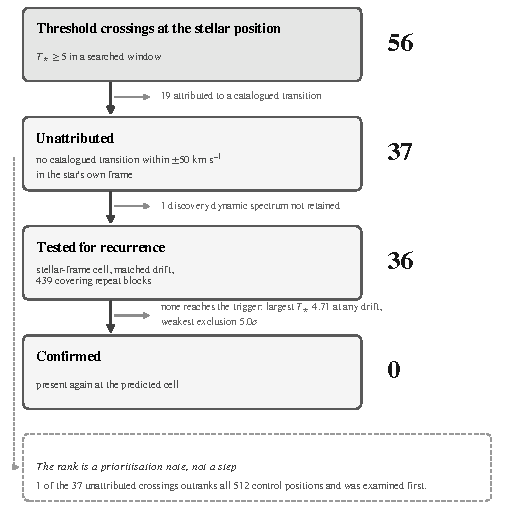
\includegraphics[width=\columnwidth]{figures/chain_v411.pdf}
\caption{What disposes of a threshold crossing. \NCross{} crossings;
\NAttributed{} attributed to a catalogued transition by the stellar-frame
mask; \NUnattributed{} unattributed, of which \RcNTested{} are tested for
recurrence against \RcNRepeatMeas{} covering repeat windows and none
recurs. The control rank is an annotation and not a step: it says which
crossing was examined first, not which survives. Every count is read from
the ledger, so the figure and Table~\ref{tab:ledger} cannot disagree.}
\label{fig:chain}
\end{figure}

%% ---------------------------------------------------------------------
%% REQUEST (results owner -> numbers owner).  Eight macros this file uses
%% that the frozen layer does not yet define, all on the adopted
%% trigger-plus-spatial-screen criterion (EirpNinetyMultA = 5.70):
%%   \EirpNinetyWinMedA                      median Class A window, W
%%   \EirpNinetySysLoA \EirpNinetySysMedA \EirpNinetySysHiA
%%                                           per system, best window, W
%%   \EirpNinetyBarnLo \EirpNinetyBarnHi     Barnard's Star, W
%%   \EirpNinetyWolfLo \EirpNinetyWolfHi     Wolf 359, W
%% The \Promote* family (\PromoteMedA, \PromoteSysMedA, ...) is the same
%% quantity on the superseded localisation criterion and is cited nowhere
%% in this file; it is still cited in 03_sample.tex and 07_conclusions.tex,
%% which must move to the names above or the paper will carry two
%% sensitivities again.  \EirpBarnLo/\EirpBarnHi/\EirpWolfLo/\EirpWolfHi
%% are nominal triggers and are no longer quoted here.
%%
%% REQUEST (results owner -> numbers owner).  tab_ledger_v403 must drop
%% nine columns: both visibility-fit epoch groups (Re/sigma, Im/sigma,
%% ctrl, twice), the epoch displacement D, the off-channel column "off",
%% and the "scr" rank flag, whose result is carried by the disposition
%% code.  Eight columns remain: star, block, band, nu, T_star, line, dv,
%% disposition.  \LedgerLegend is replaced by the caption above, so the
%% legend macro is no longer referenced.
%%
%% REQUEST (results owner -> numbers owner).  tab_maskladder.tex now has a
%% home as Table tab:maskladder in this file.  Its fourth column header
%% reads "rank-flagged", a phrase this manuscript has used in both senses;
%% please rename it to "outrank all controls" so the header cannot be read
%% as its own opposite.  The caption states the meaning meanwhile.
%%
%% REQUEST (results owner -> figures owner).  fig:chain MUST BE RE-EMITTED
%% AT SINGLE-COLUMN GEOMETRY.  It is now a \begin{figure} at \columnwidth,
%% not a figure* at 0.98\textwidth, because the section measures 6.0 pp as
%% three full-width floats and 5.0 pp with this one in a column -- the
%% overage was float packing, not words.  chain_v403.pdf is still drawn for
%% full width, so its labels are currently at about half their intended
%% size: PLEASE RE-EMIT FOR ONE COLUMN.  A six-step vertical chain reads
%% better in a column than across a page, so this is the right geometry
%% for it, but the caption, the placement and the artwork must agree and
%% today only two of the three do.  If re-emission is refused, revert this
%% float to figure*/0.98\textwidth and the section is 6.0 pp.
%%
%% REQUEST (results owner -> figures owner).  fig:bpiccontrol.
%%  - GEOMETRY CONFIRMED SINGLE COLUMN.  bpic_control.pdf is 237.6 x 280.7 pt,
%%    i.e. one column wide with the two panels stacked vertically, and the
%%    float is \columnwidth in a \begin{figure}.  Caption and placement
%%    agree; no re-emission at full width is wanted.  Panel (b) gets the
%%    full column width this way, which is what it needs.
%%  - COUNTS I WOULD NOT INVENT.  \NStageOneBpicEb (9) counts the blocks in
%%    which the star outranks every control, so it cannot also count the
%%    points drawn: the ring-wins block is by definition not one of the 9.
%%    The caption therefore says "the 9 ... and one further block" rather
%%    than giving a total.  Four macros would let it say what is drawn:
%%      \BpicPanelNCo     beta Pic CO points in panel (b)        (10)
%%      \BpicPanelNOther  other crossings drawn in grey          (39)
%%      \BpicDvCoLo \BpicDvCoHi   |dv| range of the CO crossings (12-29)
%%      \BpicDvCsLo \BpicDvCsHi   |dv| of the two CS(5-4) crossings
%%    \BpicDvLo/\BpicDvHi existed earlier today and have since been retired.
%%  - COUNTEREXAMPLE NUMBERS, requested and still absent: the ring maximum
%%    (14.13), the stellar statistic (9.68) and the number of the \NCtrl
%%    controls above the star (6) in the ring-wins block.  When they exist
%%    the caption should name that block instead of gesturing at it.
%%
%% REQUEST (results owner -> integrator).  Labels and floats deleted from
%% this file, with the files that still reference them:
%%   sec:linecost     -> sec:bpicval   (06_discussion, app_F, app_I, app_K)
%%   sec:repairedstat -> app:v409      (08_backmatter, app_A, app_M)
%%   eq:tunif         no longer defined anywhere (app_L cites it)
%%   tab:crossdelta   float deleted with the revision-history material;
%%                    app_M_repaired.tex still cites it
%%   tab:clustv409    float deleted; nothing else cites it
%%   fig:ledgervis    no longer cited (float lives in app_K)
%%   tab:hosts        no longer cited from here
%%   app:etacrvrecur  no longer cited from here (app_M still cites it)
%% ---------------------------------------------------------------------
